\chapter{Introduccion} \chapterlabel{Informe/1-Introduccion} \label{cap:Introducción}

\noindent El desarrollo de este sistema de levitación magnética surge como idea de los responsables de la cátedra Sistemas de Control, con el objetivo de disponer de una planta de control real para realizar prácticas en clase. Una primera versión de este dispositivo fue desarrollada y construída por la cátedra y los integrantes de este proyecto tuvieron la oportunidad de realizarle pruebas y modificaciones mientras cursaban la asignatura. Sin embargo, al finalizar la cursada, no se pudo lograr que el dispositivo funcionara correctamente. Por este motivo,  se propuso hacer un rediseño de todas las etapas que componen al sistema en el marco de un proyecto final.


\section{Alcance del proyecto}

\noindent El objetivo de este proyecto es diseñar un sistema de levitación magnética a partir de un electroimán de laminación normalizada con núcleo tipo “E''. Este sistema debe integrar las etapas de control de corrientes elevadas, estimación de distancia de levitación, y control de la planta. Estas dos últimas deben implementarse tanto en forma analógica como digital.

\noindent Este documento registra las etapas de diseño y modelado de todas las etapas pertenecientes al sistema, junto con su implementación circuital y simulaciones. Por último se realiza el diseño del circuito impreso que integra todas las etapas.


\section{Contexto del proyecto}

\noindent El proyecto comenzó en junio del 2020 con el objetivo de poder construir e implementar un prototipo funcional que le permita a los alumnos de la cátedra de Sistemas de Control realizar mediciones y observar el comportamiento de las distintas etapas que componen el sistema. Sin embargo, debido a los retrasos ocasionados por la pandemia de COVID-19,  la escasez de componentes a nivel mundial y de presupuesto para la construcción del circuito impreso, sumada a la  necesidad de no extender indefinidamente el proyecto, se optó por acotar el alcance sólo al diseño teórico de todas las etapas y del circuito impreso.

\noindent Por lo tanto, se espera que en el futuro pueda ser construido para que sirva como herramienta para los alumnos, de forma tal que les permita experimentar y afianzar los conceptos teóricos adquiridos durante el transcurso de la cursada.



\section{Descripción del dispositivo}

\noindent El Levitador GMI es un dispositivo capaz de mantener un objeto en suspensi\'{o}n  mediante una fuerza electromagn\'{e}tica generada por un electroim\'{a}n a una distancia $Y_0$ variable entre 3 mm y 5 mm. La distancia de separaci\'{o}n puede ser configurada por el usuario y el peso del objeto debe ser menor a 30 kg. 

\noindent El producto consta de 2 partes principales: un electroim\'{a}n y una placa de control. El electroim\'{a}n consiste en dos piezas formadas por l\'{a}minas de acero: una con forma de ``E'' que tiene un cable bobinado en su n\'{u}cleo, y otra con forma de ``I'' que es atra\'{i}da por la pieza en forma de ``E'' por medio de una fuerza electromagn\'{e}tica. Esto deja un espacio o ``\textit{gap}'' de aire entre ambas de longitud $Y_0$. Por otro lado, de la pieza en forma de ``I'' se puede colgar el objeto que se desea levantar.

\noindent El control de la fuerza electromagn\'{e}tica es realizado por una placa de control con el objetivo de mantener fija la distancia $Y_0$, a pesar de las perturbaciones externas que el sistema pueda recibir. 

\noindent Es importante aclarar que este sistema s\'{o}lo puede ejercer fuerza verticalmente, por lo tanto no puede controlar la posici\'{o}n horizontal.


\noindent El sistema est\'{a} conformado por los bloques que se muestran en la figura \ref{fig:img_modelo_bloques1}.. Se utilizan dos controladores distintos: uno anal\'{o}gico y otro digital. Cada uno de ellos se compone de un compensador y un estimador de posici\'{o}n.  El usuario decidir\'{a} cual de estas implementaciones ejercer\'{a} el control mediante la utilizaci\'{o}n de un \textit{switch}, por lo que solo una estar\'{a} activa al mismo tiempo. El sistema anal\'{o}gico est\'{a} formado por un conjunto de componentes pasivos y amplificadores operacionales, mientras que el digital est\'{a} basado en un microcontrolador re-programable. Adem\'{a}s, el estimador de posici\'{o}n se encarga de  entregar una tensi\'{o}n proporcional al \textit{gap }de aire real en funci\'{o}n de  la corriente que circula por el electroim\'{a}n.


\begin{figure}[H]
	\centering
	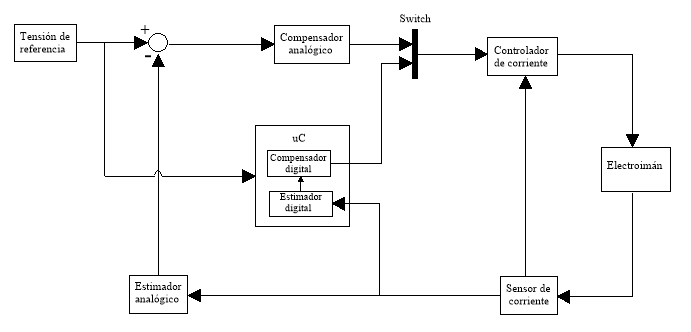
\includegraphics[scale=0.5]{diagrama-en-bloques-del-sistema.png}
	\caption{Diagrama en bloques del sistema}
	\label{fig:img_modelo_bloques1}
\end{figure}


\noindent El usuario puede modificar el gap de aire que desea mediante un potenci\'{o}metro presente en la placa de control, que entrega una tensi\'{o}n proporcional a la misma. Tanto la implementaci\'{o}n anal\'{o}gica como la digital reciben como entrada esta tensi\'{o}n. Luego, es comparada con la estimaci\'{o}n y se utiliza como entrada para el compensador.

\noindent La funci\'{o}n del compensador es garantizar la estabilidad del sistema. Esto lo logra al modificar la referencia del controlador de corriente mediante una acci\'{o}n de control. El controlador de corriente se encarga de proveer corriente al electroim\'{a}n de forma tal que le permita generar la fuerza electromagn\'{e}tica necesaria para mantener el gap de aire. 

\noindent Por otra parte, se utiliza un software de PC para modificar los coeficientes de la implementaci\'{o}n digital.